\documentclass[letterpaper,11pt]{article}
\usepackage{setspace} % For double-spaced text
\usepackage{geometry}
\usepackage{multicol}
\usepackage{graphicx}
\usepackage{float}
\usepackage{mathrsfs}

\graphicspath{ {timing_study.png} }
% \doublespacing

\title{CMSE 401 - Homework 1}
\author{Jack Hamel}

\topmargin-2cm     %I recommend adding these three lines to increase the
\textwidth16.5cm   %amount of usable space on the page (and save trees)
\textheight23.5cm
\oddsidemargin0cm

\begin{document}

\maketitle

\section{Implementation}

The wave function algorithm outlined in the homework one assignment was implemented in both C++ and Python 3.  The algorithm in the C++ code follows the one proposed in the assignment as closely as possible and the Python code has an augmented version to decrease run time.  The C++ version uses standard libraries and the Eigen linear algebra library and the Python version uses Numpy and Matplotlib.  The Python code is verifiably correct and is the version I wish the grading of this assignment to be based on.  

The C++ code does not give the same results as the Python code, although they do not seem to be overly erroneous.  The differing results are unlikely to be due to accumulating numerical noise or implementation/compilatiion differences because the discrepancies are too large; however, the error (defined here as the difference between the two result sets) between results increases with each time step.  This leads me to believe the error is caused by a minute difference in the two codes that compounds over time.  Beyond this conclusion, I have no additional ideas as to why this is the case other than a bug that I was unable to find.  

As mentioned before, the algorithm of the Python code does not exactly follow the one outlined in the assignment directions.  First, a number of lines were added to save data to use in the animation of the simulation output.  These can be turned off by setting the animate variable equal to 0.  In order to speed up the code, I worked to remove the nested for loop that results from following the assignment directions.  This was done by taking advantage of the ability to operate on elements of Numpy arrays without a loop.  Second, I removed the use of a vector, reducing the storage needed and time spent alocating data.  Last, I removed redundancies in the algorithm such as looping through the first time step and setting the acceleration at line ends equal to zero.  These changes resulted in changing a code that took too long for my patience to run with $nx=500$ and $nt=1e6$ to it running in under 20 seconds.  
\section{Timing Study}

To benchmark the performance of the python code, I ran the simulation for all combinations of the following degrees of freedom (nx) and number of time steps (nt): $nx \subset [100, 500]$ and $nt \subset [1e2, 1e3, 1e4, 1e5, 1e6]$.  This was done using an additional python script that ran these combinations six times each and averaged the time for each run.  The figure below shows how the duration of the simulations scales as the degrees of freedom and number of timesteps are changed.
\begin{figure}[H]
  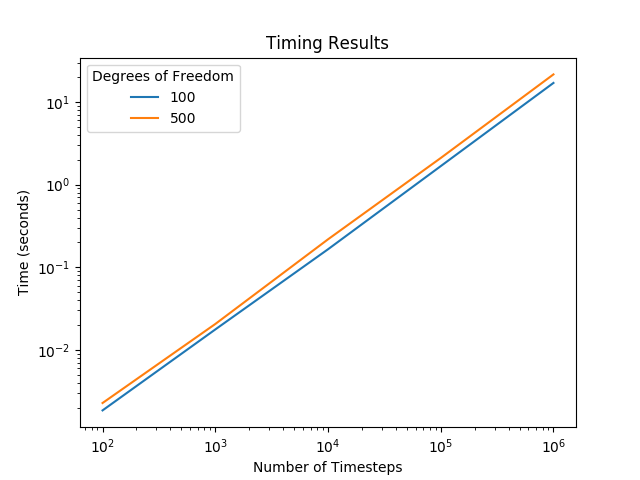
\includegraphics[scale=0.9]{timing_results.png}
  \caption{Scaling of the wave function simulation}
\end{figure}

When $nx=500$ and $nt=1e6$ run time $= 17.912 seconds$.
\newline

The Computer Specifications used during this study are as follows:

Processor: Intel Core i3-4030U @ 1.90GHz w/ 4 cores (1 core used)

Graphics: Intel Haswell Mobile

Memory: 3.7 GB

OS: Ubuntu 18.04.1 LTS 64-bit


\section{Instructions}

I will submit two versions of the Python code with this project.  One version is titled $\texttt{time\_study.py}$ and when ran generates the data used to create the scaling plot shown above.  This version is used to gather timing data.  The second version is titled $\texttt{hw1.py}$ and will be useful in grading the project.  It is the same code, but will generate an animation showing the 1D wave equation, rather than gather timing data.

To run this code, you will need Python 3 installed and access to the Numpy and Matplotlib libraries.  To get these, follow the instructions on how to download and install Anaconda, which includes all of the software you will need.  Since both versions of my Python code use graphics, I recommend running the IDE called Spyder that is included with Anaconda.  Running the code within this program will give you access to the graphical outputs.  Use the following link to get Anaconda: https://www.anaconda.com/download/

The C++ code submitted is titled $\texttt{hw1\_2.cpp}$.  This code requires the non-standard C++ library called Eigen.  You can download the source code for Eigen from the link below.  Once downloaded, you simply extract the contents of the downloaded file to a location of your choice.  To compile the code you need to run $\texttt{g++ -I /path/to/Eigen hw1\_2.cpp}$  The -I option means you want to include the following path during compiling.  You can add The Eigen source code to your environment path and neglect using the -I option.  To run the code, use the command $/texttt{./a.out}$ where $/texttt{a.out}$ is the default executable name generated when compiling using GCC.  Eigen source code can be found here: http://eigen.tuxfamily.org/index.php?title=Main\_Page\#Download
\end{document}
